\documentclass[12pt]{article}
\usepackage{mathtools}
\usepackage{amsthm,amssymb}
\usepackage{verbatim,comment,xcolor,graphicx,hyperref}
%\usepackage[papersize={4.5in, 6.2in}, width=4.13in, height=5.83in, vcentering, centering]{geometry} % Kindle-size pages
\usepackage[left=1.0in,right=1.0in,top=1.0in,bottom=1.0in]{geometry} % never use the anysize package!
\usepackage{mathpazo}

\newcommand{\degs}[1]{\textsuperscript{$\circ$}#1}
\definecolor{footlineblue}{rgb}{0.392,0.706,0.941}

\parskip=12pt
\parindent=0pt

% tikz stuff and other macros
% Jesse Hamner
% 2013--2024

\usepackage{tabularx}

\newcolumntype{R}[2]{%
    >{\adjustbox{angle=#1,lap=\width-(#2)}\bgroup}%
    l%
    <{\egroup}%
}


% make a few color defs:
\definecolor{rltbrightred}{rgb}{1,0,0}
\definecolor{rltred}{rgb}{0.75,0,0}
\definecolor{rltdarkred}{rgb}{0.5,0,0}
\definecolor{rltbrightgreen}{rgb}{0,0.75,0}
\definecolor{rltgreen}{rgb}{0,0.5,0}
\definecolor{rltdarkgreen}{rgb}{0,0.25,0}
\definecolor{rltbrightblue}{rgb}{0,0,1}
\definecolor{rltblue}{rgb}{0,0,0.75}
\definecolor{rltdarkblue}{rgb}{0,0,0.5}
%\definecolor{webred}{rgb}{0.5,.25,0}
\definecolor{webblue}{rgb}{0,0,0.75}
\definecolor{webgreen}{rgb}{0,0.5,0}
\definecolor{lightgray}{gray}{0.9}
\definecolor{medgray}{gray}{0.6}
\definecolor{footlineblue}{rgb}{0.392,0.706,0.941}
\definecolor{darkgreen}{rgb}{0.00,0.50,0.00}
\definecolor{gray50}{gray}{0.50}
\definecolor{gray95}{gray}{0.95}
\definecolor{webred}{rgb}{0.75,0,0.0}

\renewcommand{\thefootnote}{\fnsymbol{footnote}}
\newcommand{\sep}{1mm}
\newcommand{\negsep}{-4mm}
\newcommand{\widesep}{7mm}
\newcommand{\thisscale}{0.6}
\newcommand{\grr}{\rowcolor{gray!15}}

\newcommand{\+}{\item}		% easier than typing \item a lot
\newcommand{\bi}{\begin{itemize}}
\newcommand{\ei}{\end{itemize}}
\newcommand{\bd}{\begin{description}}
\newcommand{\ed}{\end{description}}
\newcommand{\be}{\begin{enumerate}}
\newcommand{\ee}{\end{enumerate}}
\newcommand{\rr}{\raggedright}

\newcommand{\cb}{\cellcolor{black!35}}

\newcommand{\ckb}{\item[$\square$]} % list checkboxes (requires marvosym)

% A command that makes a uniform box around a paragraph. 
% It's a minipage environment, which means it doesn't support some commands.
\newcommand{\stbox}[2]{
	\begin{center}
	\fbox{
		\begin{minipage}[c]{#1}{
		\noindent #2
		}
		\end{minipage}
	}
	\end{center}
}


% A series of macros that enable programmatic of drawing stylized
% ions, protons, or electrons.
% Supports,  e.g., richer drawings of capacitors or
% current flowing in wires:

\newcommand{\ionradius}{0.06} % TODO should make it possible to change this too

\newcommand{\drawion}[4]{
		\draw [black, very thin] (#1,#2) circle [radius=#3];
		\node[scale=0.3, thick ] at (#1,#2) {#4};
}

\newcommand{\posion}[3]{
		\drawion{#1}{#2}{#3}{$+$}
		}

\newcommand{\negion}[3]{
		\drawion{#1}{#2}{#3}{$-$}
		}

\newcommand{\horizionarray}[4]{
	\newdimen\len
	\len=#1 cm
	\advance\len by -0.4cm
	\drawion{\len}{#2}{\ionradius}{#4}
	\advance\len by 0.15cm
	\drawion{\len}{#2}{\ionradius}{#4}
	\advance\len by 0.15cm
	\drawion{\len}{#2}{\ionradius}{#4}
	\advance\len by 0.2cm
	\drawion{\len}{#2}{\ionradius}{#4}
	\advance\len by 0.15cm
	\drawion{\len}{#2}{\ionradius}{#4}
	\advance\len by 0.15cm
	\drawion{\len}{#2}{\ionradius}{#4}
}

\newcommand{\vertionarray}[4]{
	\newdimen\len
	\len=#2 cm
	\advance\len by -0.4cm
	\drawion{#1}{\len}{\ionradius}{#4}
	\advance\len by 0.15cm
	\drawion{#1}{\len}{\ionradius}{#4}
	\advance\len by 0.15cm
	\drawion{#1}{\len}{\ionradius}{#4}
	\advance\len by 0.2cm
	\drawion{#1}{\len}{\ionradius}{#4}
	\advance\len by 0.15cm
	\drawion{#1}{\len}{\ionradius}{#4}
	\advance\len by 0.15cm
	\drawion{#1}{\len}{\ionradius}{#4}
}



% Nokia 84 x 48 pixel LCD screen (usually model number 5110 or 3310)
\newcommand{\drawnokiagrid}{
\draw[step=1cm,blue!30,very thin] (0,0) grid (6,8);
\foreach \x in {0,1,2,3,4,5}
	\draw (\x cm, 0pt) -- (\x cm, -3pt) node[anchor=north] {$\x$};
\foreach \y in {1,2,3,4,5,6,7,8}
	\draw (0pt, \y cm) -- (-3pt, \y cm) node[anchor=east] {$\y$};
}


% part of the Nokia grid set of commands
\newcommand{\msqo}[3]{
\def\mycmd{#3}

\if\mycmd1
	\msq{#1}{#2}{black!65}
\else
	\msq{#1}{#2}{white}
\fi
}


% part of the Nokia grid set of commands
\newcommand{\msq}[3]{
\edef\myx{#1}
\pgfmathparse{\myx+1.0}
\edef\myxtwo{\pgfmathresult}
\edef\myy{#2}
\pgfmathparse{\myy+1.0}
\edef\myytwo{\pgfmathresult}
\fill[#3] (\myx,#2) rectangle (\myxtwo,\myytwo);}


% part of the Nokia grid set of commands
\newcommand{\mcol}[9]{
\msqo{#1}{#2}{#3}
\msqo{#1}{#4}{#5}
\msqo{#1}{#6}{#7}
\msqo{#1}{#8}{#9}
}


% part of the Nokia grid set of commands
\newcommand{\hexlabel}[5]{
\node[rotate=90] at (0.5,-1) {\Large\texttt{#1}};
\node[rotate=90] at (1.5,-1) {\Large\texttt{#2}};
\node[rotate=90] at (2.5,-1) {\Large\texttt{#3}};
\node[rotate=90] at (3.5,-1) {\Large\texttt{#4}};
\node[rotate=90] at (4.5,-1) {\Large\texttt{#5}};
}



% drawing cubes using TikZ:
\newcommand{\makecube}[2]{
\begin{tikzpicture}[xscale=#2,yscale=#2]
\foreach \x in{0,...,#1}
{   \draw (0,\x ,#1) -- (#1,\x ,#1);
    \draw (\x ,0,#1) -- (\x ,#1,#1);
    \draw (#1,\x ,#1) -- (#1,\x ,0);
    \draw (\x ,#1,#1) -- (\x ,#1,0);
    \draw (#1,0,\x ) -- (#1,#1,\x );
    \draw (0,#1,\x ) -- (#1,#1,\x );
}
\end{tikzpicture}
}


% Draw faux-3D squares or cubes:
\newcommand{\makeplate}[3]{
\begin{tikzpicture}[xscale=#3,yscale=#3]

\foreach \x in {0,...,#1}
{
	\filldraw[gray95, fill=gray95, line width=0.0cm] (0,#1,0) -- (0,#1,#2) -- (#1,#1,#2) -- (#1,#1, 0) -- (0,#1,0) -- cycle;
	\filldraw[gray50, fill=gray50, line width=0.0cm] (#1,#1,0) -- (#1,#1,#2) -- (#1,0,#2) -- (#1,0, 0) -- (#1,#1,0) -- cycle;
}

\foreach \x in{0,...,#1}
{   \draw (0,\x ,#2) -- (#1,\x ,#2);
    \draw (\x ,0,#2) -- (\x ,#1,#2);
	\draw (#1,\x ,#2 ) -- (#1,\x ,0);
    \draw (\x ,#1,#2 ) -- (\x ,#1,0);
}

\foreach \x in {0,...,#2}
{
    \draw(#1,0,\x  ) -- (#1,#1,\x );
    \draw(0,#1,\x  ) -- (#1,#1,\x );
}

\foreach \x in{1,...,#1}
{
\node[align=left] at (\x-0.5,#1-0.5,#2) {\x};
}

\foreach \x in{#1,...,2}
{
\node[align=left] at (0.5,#1-\x+0.5,#2) {\x};
}

%\draw[webred, thick](0,0,0) -- (0,0,#2);
%\draw[webblue, thick](0,0,0) -- (#1,0,0);
%\draw[darkgreen, thick](0,0,0) -- (0,#1,0);

\end{tikzpicture}
}


% Draw a line of faux-3D shaded blocks using TikZ:
\newcommand{\blockline}[2]{
\begin{tikzpicture}[xscale=#2,yscale=#2]

\filldraw[fill=gray95, ultra thin] (0,1,0) -- (0,1,1) -- (#1,1,1) -- (#1,1, 0) -- (0,1,0) -- cycle;
\filldraw[fill=gray50, ultra thin] (#1,1,0) -- (#1,1,1) -- (#1,0,1) -- (#1,0, 0) -- (#1,1,0) -- cycle;

\draw (0,1,0 ) -- (#1,1,0); % top line
\draw (#1,1,1) -- (#1,1,0);
\draw (#1,0,1) -- (#1,1,1);
\draw (0,1, 1) -- (#1,1,1);
\draw (0,0,1 ) -- (#1,0,1);

\foreach \x in{0,...,#1}
{   
    \draw (\x ,0,1) -- (\x ,1,1 ); % straight vertical lines    
    \draw (\x ,1,1) -- (\x ,1,0 );
}

\foreach \x in{1,...,#1}
{
	\node[align=left] at (\x-0.5,0.5,1) {\x};
}

\end{tikzpicture}
}


% make a blank line under which, e.g., someone could write an unknown answer:
\newcommand{\makeblank}[1]{
\underline{\makebox[#1][l]{}}
}


% tilt the text atop a table row at an angle:
\newcommand*\rot{\multicolumn{1}{R{55}{1.2ex}}}% no optional argument here, please!


\newcommand{\adderblock}[3]{

	\begin{scope}

	\draw (0,#1)
	  [xshift = 2.5cm]
	  node[one bit adder, scale=0.75](fa#2){}
	  node[xshift=0.75cm, yshift=1cm](fa#2carrylabel){\footnotesize $Carry_#3$}
  	  node[ocirc, xshift=1.5cm, label={[label distance=0mm]0:$Sum_#3$}](fa#2sum){}
	;

    \draw (0.5,#1)
 	  [yshift=-0.65cm] 
	  node[american xor port](axorb#2){}
	  node[ocirc, xshift = -2.2cm, yshift = -0.28cm](axorb#2node){}
   	  node[xshift = -2.6cm, yshift = 0mm](){{\color{red}$A_{#3}$}}
	  node[xshift = 0.2cm, yshift = 6mm] {{\footnotesize{$XOR_{#3}$}}}
   	  node[ocirc, xshift = -4.5cm, yshift = 0.32cm](m#2node){}
	  node[xshift = -4.0cm, yshift = 0.6cm, color=rltred]{\color{rltred}$M_{#3}$}
	;
 
    \draw (0,#1)
	  [yshift=0.65cm]
	  node[ocirc, xshift = -2.0cm](b#2node){}
   	  node[xshift = -2.3cm, yshift = 3mm](){{\color{blue}$B_{#3}$}}
    ;
  
    \draw (0,#1)
	  [color=blue] 
	  (b#2node) -- (fa#2.lpin 1) 
	;
  
    \draw
	  [color=rltred] 
	  (m#2node) -- (axorb#2.in 1) 
	;

    \draw (0,#1)
	  (axorb#2node) -- (axorb#2.in 2)
	  (fa#2.rpin 1) -- (fa#2sum)
	;
	
    \draw(0, #1)[color=brown, very thick]
      (axorb#2.out) -- (fa#2.lpin 2)
    ;
    
  \end{scope}
}



% Half Adder Symbol:
\newcommand{\halfadder}{
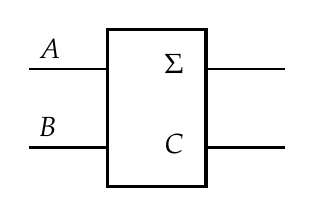
\begin{tikzpicture}

\draw [very thick] (0,0) -- (1.25,0) -- (1.25,2) -- (0,2) -- cycle;
\draw [thick] (-1,0.5) -- (0,0.5);
\draw [thick] (-1,1.5) -- (0,1.5);
\draw [thick] (1.25,0.5) -- (2.25,0.5);
\draw [thick] (1.25,1.5) -- (2.25,1.5);

\node[xshift=-10mm, yshift=20mm, anchor= north west] {$A$};
\node[xshift=-10mm, yshift=10mm, anchor= north west] {$B$};
\node[xshift=6mm, yshift=18mm, anchor= north west] {$\Sigma$};
\node[xshift=6mm, yshift=8mm, anchor= north west] {$C$};

\end{tikzpicture}
}


% Full Adder Symbol:
\newcommand{\fulladder}{
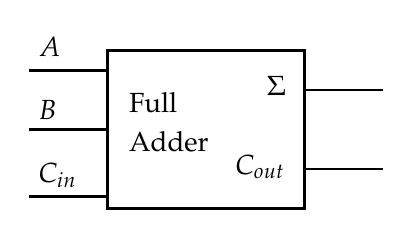
\begin{tikzpicture}

\draw [very thick] (0,0) -- (2.5,0) -- (2.5,2) -- (0,2) -- cycle;
\draw [thick] (-1,0.15) -- (0,0.15);
\draw [thick] (-1,1.0) -- (0,1.0);
\draw [thick] (-1,1.75) -- (0,1.75);

\draw [thick] (2.5,0.5) -- (3.5,0.5);
\draw [thick] (2.5,1.5) -- (3.5,1.5);

\node[xshift=-10mm, yshift=23mm, anchor= north west] {$A$};
\node[xshift=-10mm, yshift=15mm, anchor= north west] {$B$};
\node[xshift=-10mm, yshift=7mm, anchor= north west] {$C_{in}$};

\node[xshift=19mm, yshift=18mm, anchor= north west] {$\Sigma$};
\node[xshift=15mm, yshift=8mm, anchor= north west] {$C_{out}$};
\node[xshift=1.5mm, yshift=16mm, anchor= north west] {Full};
\node[xshift=1.5mm, yshift=11mm, anchor= north west] {Adder};

\end{tikzpicture}
}

\graphicspath{{../images/}}

\begin{document}

\thispagestyle{empty}
\date{}
\title{Discrete Logic Gates Guide}
\author{Jesse Hamner}


\maketitle

\begin{abstract}
This guide contains the parts lists and schematics for each of the logic gates included in the repository. All fundamental logic gates are included, as are several more complex gates. These gates are in no way designed to be efficient or cost-effective; they are intended as functional, educational-only components. Some of the boards require surface-mount components, to reduce cost and size, but none of the discrete logic gates do. That is, some of the infrastructure pieces, and ``move things along more smoothly'' pieces, require SMD soldering, but workarounds for these units exist, using through-hole components and a solderless breadboard (see text for more). The bills of materials (BOMs) were created with cost in mind, but very few through-hole P-type MOSFETs are available, and they cost over USD\$0.30 apiece, as of this writing. The N-type MOSFETs are much cheaper, but the costs can add up quickly if you are building XOR gates. Especially because of the cost of through-hole P-type MOSFETS, some components will be SMD-only until demand rises for through-hole solderable versions.\\
~\\
\textbf{Keywords:} STEM; education; electronics; elementary education; soldering.

\end{abstract}

\begin{center}
\fbox{
\includegraphics[scale=0.09, clip=true, trim = 100 200 500 0]{soldering2.jpg}
}

A second grader soldering through-hole headers and components.
\end{center}
\clearpage 

~
\vfill

\begin{center}
\includegraphics[scale=1.0]{by-nc-nd.png}

This work is licensed under a {\color{webblue}\href{https://creativecommons.org/licenses/by-nc-sa/4.0/}{Creative Commons Attribution-NonCommercial-ShareAlike 4.0 International License.}}
% Attribution-NonCommercial-ShareAlike 4.0 International (CC BY-NC-SA 4.0)
\end{center}


\newpage


\section{OR Gate} Making an OR gate is almost trivially easy -- you can even make it without 
transistors. The simplest OR gate is two inputs, each into a diode, and the diodes tied together 
as an output. It's not a very good OR gate, but it works. 
Transistor-transistor logic (TTL) OR gates are more recognizable, but BJT transistors need a 
significant amount of resistance on the gate and the output to drag the voltage low enough to 
count as a zero. Typically, a CMOS OR gate is a NOR gate coupled with a NOT gate, since both 
of these gates can be made with CMOS circuits and therefore save energy and reduce heat.



\section{AND Gate}

Two versions exist: MOSFET and TTL. Similar to the OR gate, CMOS AND gates are usually NAND and NOT gates on the output.
The TTL version is only for demonstration. 

\section{NOT Gate}

The NOT, NOR, and NAND gates all use {\color{webblue}\href{https://en.wikipedia.org/wiki/CMOS}{Complementary Metal Oxide Semiconductor}} (CMOS) construction, because of the low power consumption and clarity of output voltages. The NOT gate, in particular, is very elegant in CMOS construction: when the input line is low (logic 0), the P-type transistor is open and the N-type transistor is closed, meaning all voltage is available via the P-type FET, cannot flow to ground because the N-type FET is blocked off, and so goes to the output. The reverse (the \emph{complement}) happens when the input line is high (logic 1): the P-type gate is closed, and the N-type gate is open, preventing the flow of current from the voltage input, and exposing ground voltage (zero volts) to the output.

\begin{center}
\input{../include/NOTgateBOM.tex }
\end{center}

\section{NOR Gate}

CMOS

\section{NAND Gate}

CMOS

\section{XOR Gate}

While it is possible to make an XOR gate with less than 12 transistors, this version uses 12, because it becomes possible to see the individual gates in the schematic and even the board layout. This board also uses CMOS topology, which improves its speed and output response.

\begin{figure}[!hb]
\begin{center}
\fbox{
\includegraphics[scale=0.20]{xorgatelayout.png}
}
\medskip
\caption{A 12-transistor eXclusive-OR (XOR) gate. This design uses complementary transistors (CMOS).}
\label{fig:xor1}
\end{center}
\end{figure}


\section{Full Adder}

Uses SMD components, with one logic gate per IC. While it is possible to get full adders on a single chip, these boards maintain the relative ease of ``following the electrons" from gate to gate, without the cost or size requirements to achieve 4 or more full adders with discrete transistors. Participants would be well-served to make at least one full adder from discrete-component gates, just to prove that it works to themselves, but perhaps use these full adder boards to make the ``calculator.''

The added difficulty of SMD soldering is obvious, and including the SMD design reflects a space- and cost-conscious approach, rather than the expectation that all novices should be able to solder surface-mount components. These are not the easiest to surface mount, but the author has had success hand-soldering 0603 and even 0402-sized components without a microscope, so with practice, the larger 0805 and SOT-23 pattern components are not a challenge.

\section{Toggle Switch Board}

a bank of 4 toggle switches, with LED indicators built in. This design requires SMD soldering, but can be duplicated without much pain on a breadboard. Furthermore, the LED indication can be omitted with no loss of functionality. In other words, while it is easier to solder the SMD components first, it is at least possible to solder them after installing the switches. These designs include some ``nice-to-haves" like  capacitors on the data inputs and power supply. Especially in winter, stray capacitance can create some odd effects, so these extra components provide a measure of reliability and help ensure sane behavior of the circuits.

\begin{tabular}{l l l p{2.9in} } 
\hline\\
\textbf{Part} & \textbf{Value} & \textbf{Package} & \textbf{Description} \\[3mm]
\hline\\\\[-7mm]
$\square$ C1 & 0.1$\mu F$ & C0805 & capacitor \\
$\square$ C2 & 0.1$\mu F$ & C0805 & capacitor \\
$\square$ C3 & 0.1$\mu F$ & C0805 & capacitor \\
$\square$ C4 & 0.1$\mu F$ & C0805 & capacitor \\
$\square$ JP1 &  & $1 \times 2$ Header & Standard 2-pin 0.1 header \\
$\square$ JP2 &  & $1 \times 4$ Header & Header 4 \\
$\square$ LED0 &  & 0805 & LED \\
$\square$ LED1 &  & 0805 & LED \\
$\square$ LED2 &  & 0805 & LED \\
$\square$ LED3 &  & 0805 & LED \\
$\square$ Q0 & 2N2222 & SOT23 & NPN TRANSISTOR \\
$\square$ Q1 & 2N2222 & SOT23 & NPN TRANSISTOR \\
$\square$ Q2 & 2N2222 & SOT23 & NPN TRANSISTOR \\
$\square$ Q3 & 2N2222 & SOT23 & NPN TRANSISTOR \\
$\square$ R1 & 330$\Omega$ & M0805 & resistor \\
$\square$ R2 & 330$\Omega$ & M0805 & resistor \\
$\square$ R3 & 330$\Omega$ & M0805 & resistor \\
$\square$ R4 & 330$\Omega$ & M0805 & resistor \\
$\square$ R5 & 1K & M0805 & resistor \\
$\square$ R6 & 1K & M0805 & resistor \\
$\square$ R7 & 1K & M0805 & resistor \\
$\square$ R8 & 1K & M0805 & resistor \\
$\square$ S0 & SPDT & SLIDESWITCHSPDT & Single pole single-throw slide switch \\
$\square$ S1 & SPDT & SLIDESWITCHSPDT & Single pole single-throw slide switch \\
$\square$ S2 & SPDT & SLIDESWITCHSPDT & Single pole single-throw slide switch \\
$\square$ S3 & SPDT & SLIDESWITCHSPDT & Single pole single-throw slide switch \\
\end{tabular}


\section{8-LED Indicator}

Again, this indicator bank uses surface mount components, primarily to economize on cost of transistors and PCBs. It is very easy to rig up many LED indicators on a solderless breadboard, should SMD soldering be daunting to the end-users. However, as above, hand-soldering these components is not unreasonably hard. This board is available here because of its general usefulness, and because it appears in some document figures. Admittedly, these boards are best soldered in a reflow oven, using solder paste and a solder stencil. See Figure \ref{fig:smds} as evidence a 9-year-old can do that with some care and patience.

\begin{figure}[!hb]
\begin{center}
\fbox{
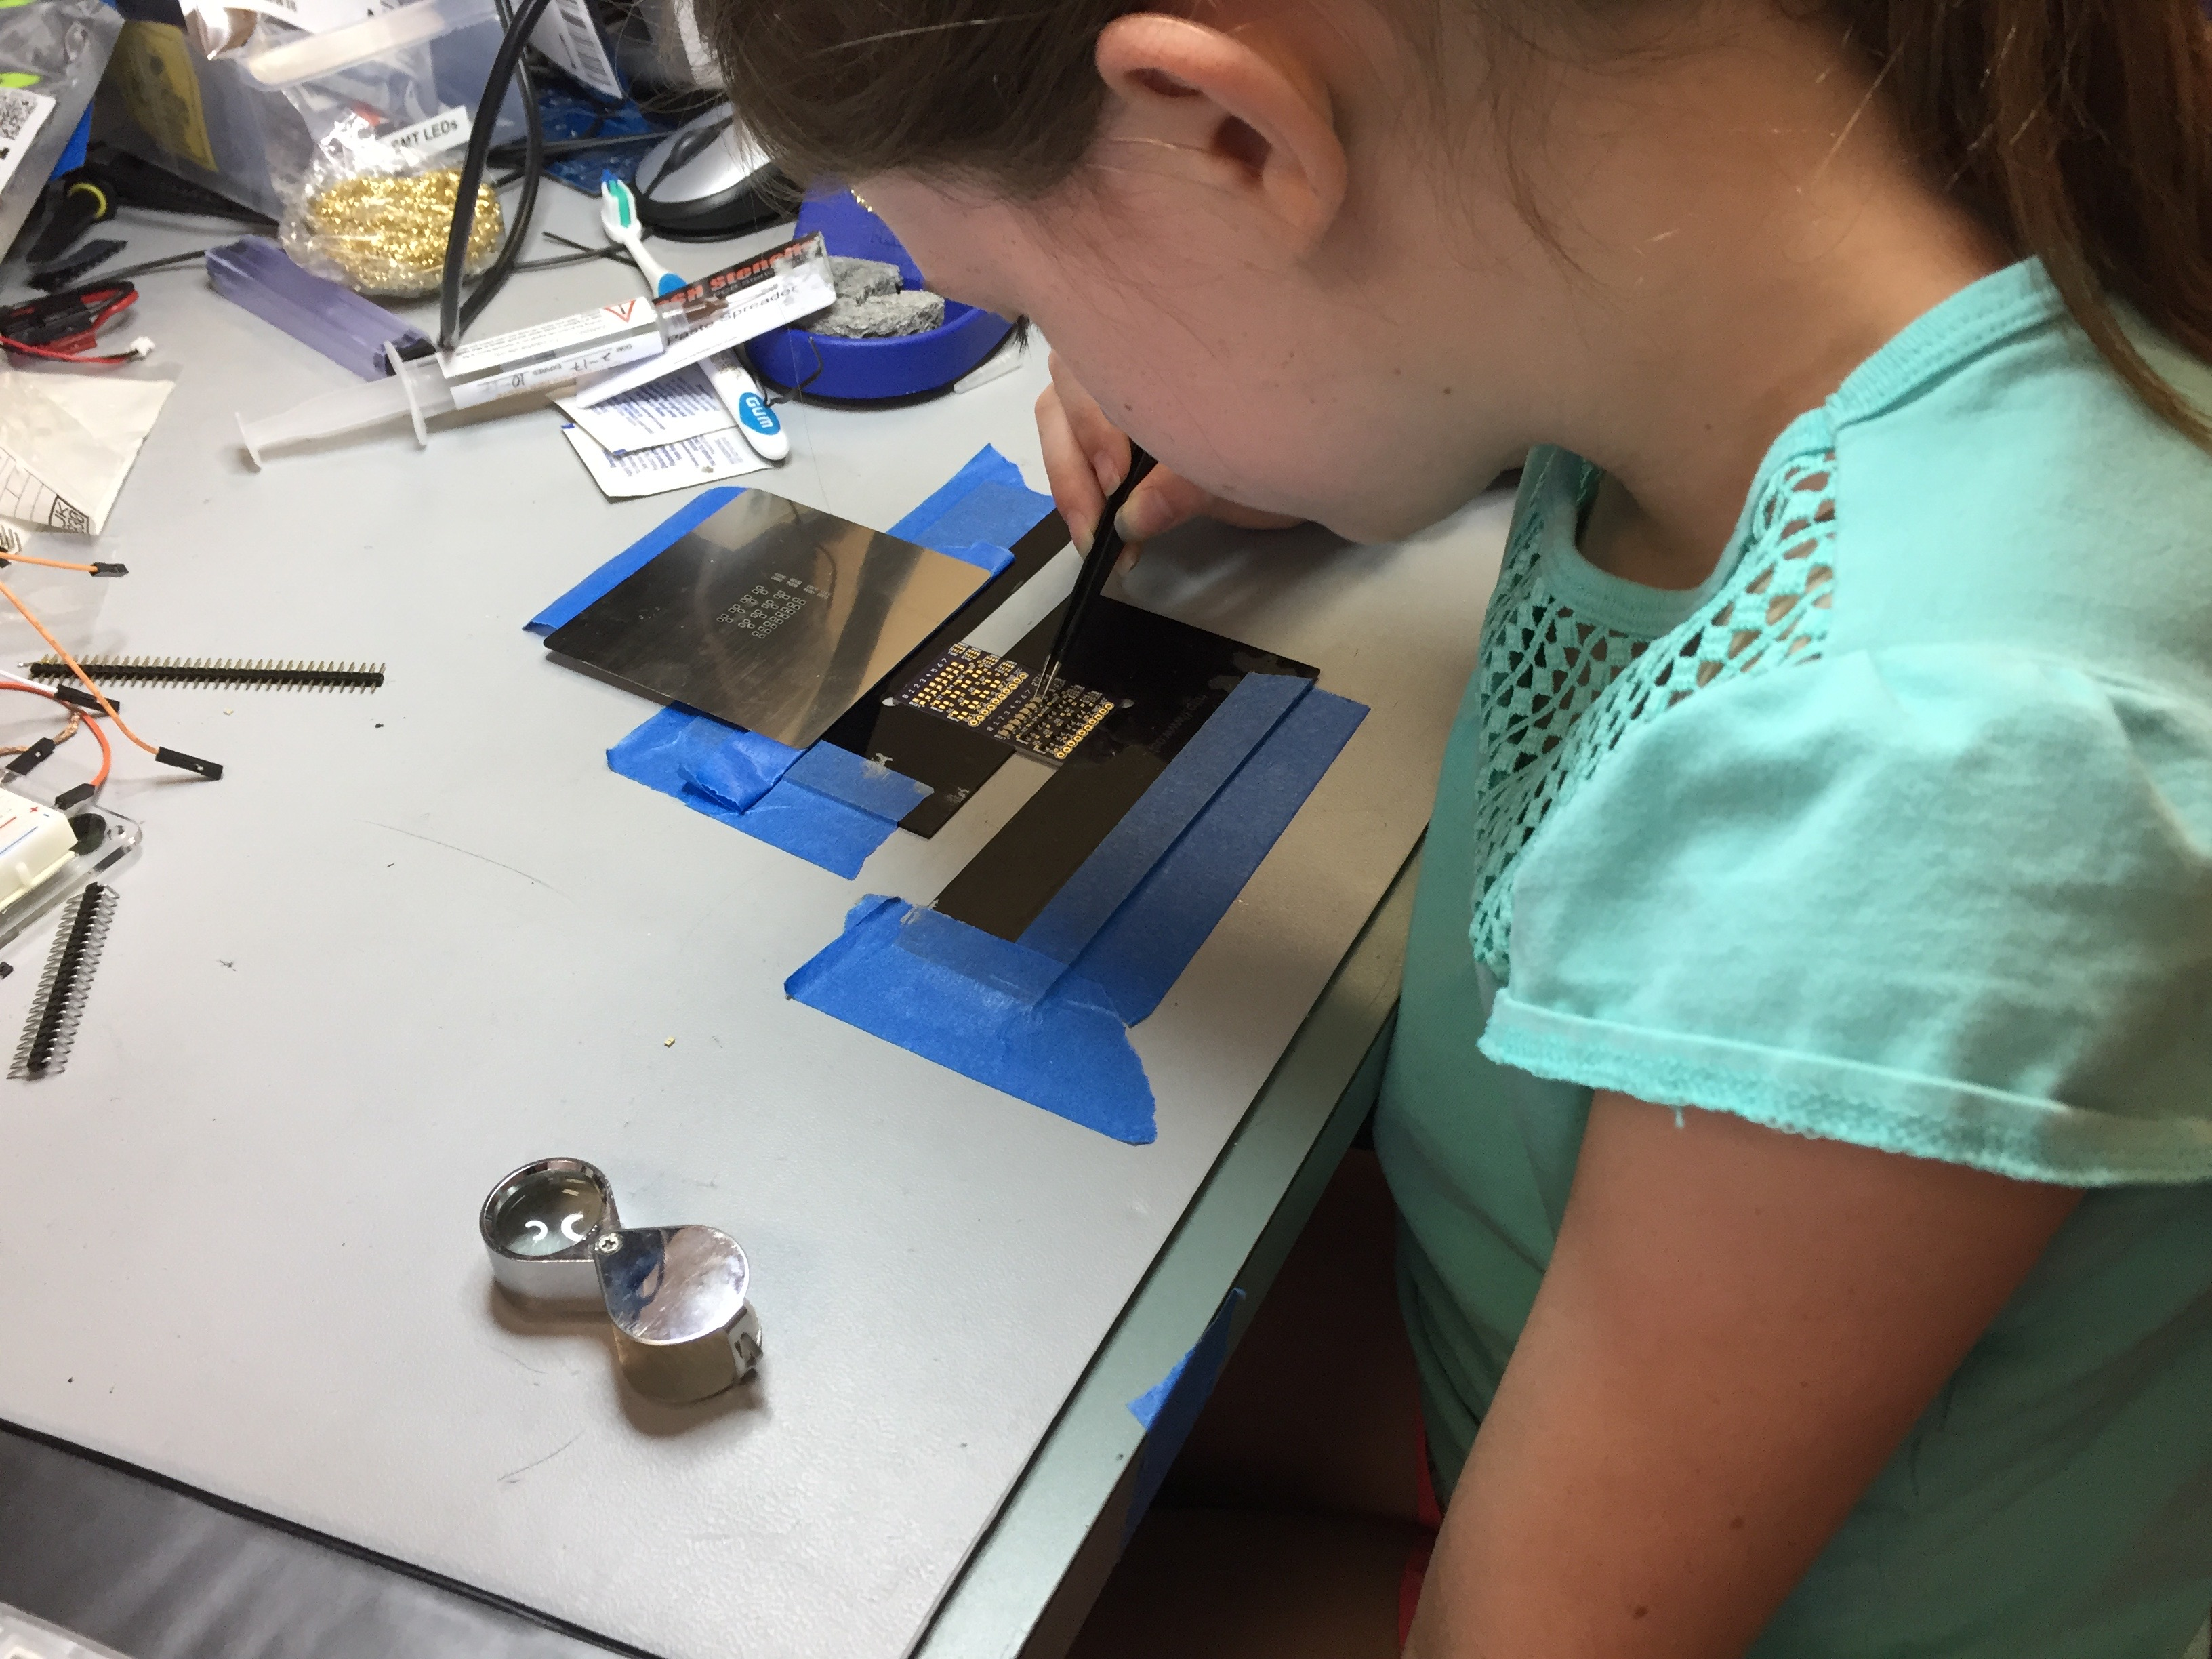
\includegraphics[scale=0.08]{placingSMDs.jpg}
}
\medskip
\caption{An elementary school student placing 0805 and SOT-23 components on to a PCB with solder paste already applied through a metal stencil. The solder paste helps hold components in place until they are soldered in a reflow oven. Reflow ovens can be obtained as cheaply as USD 200.}
\label{fig:smds}
\end{center}
\end{figure}

\begin{tabular}{l l l p{3.5in} } 
\hline\\
\textbf{Part} & \textbf{Value} & \textbf{Package} & \textbf{Description} \\[3mm]
\hline\\\\[-7mm]
$\square$ JP1 & M10LOCK & 1X10\_LOCK & Header 10 \\
$\square$ LED0 & GRN & CHIP-LED0805 & LED \\
$\square$ LED1 & GRN & CHIP-LED0805 & LED \\
$\square$ LED2 & GRN & CHIP-LED0805 & LED \\
$\square$ LED3 & GRN & CHIP-LED0805 & LED \\
$\square$ LED4 & GRN & CHIP-LED0805 & LED \\
$\square$ LED5 & GRN & CHIP-LED0805 & LED \\
$\square$ LED6 & GRN & CHIP-LED0805 & LED \\
$\square$ LED7 & GRN & CHIP-LED0805 & LED \\
$\square$ Q1 & 2N3904 & SOT23 & BJT NPN transistor \\
$\square$ Q2 & 2N3904 & SOT23 & BJT NPN transistor \\
$\square$ Q3 & 2N3904 & SOT23 & BJT NPN transistor \\
$\square$ Q4 & 2N3904 & SOT23 & BJT NPN transistor \\
$\square$ Q5 & 2N3904 & SOT23 & BJT NPN transistor \\
$\square$ Q6 & 2N3904 & SOT23 & BJT NPN transistor \\
$\square$ Q7 & 2N3904 & SOT23 & BJT NPN transistor \\
$\square$ Q8 & 2N3904 & SOT23 & BJT NPN transistor \\
$\square$ RA1 & 220$\Omega$ & CAY16-J4 & Resistor Network with 4 resistors, 1206 package \\
$\square$ RA2 & 100K & CAY16-J4 & Resistor Network with 4 resistors, 1206 package \\
$\square$ RA3 & 220$\Omega$ & CAY16-J4 & Resistor Network with 4 resistors, 1206 package \\
$\square$ RA4 & 100K & CAY16-J4 & Resistor Network with 4 resistors, 1206 package \\
\end{tabular}




\end{document}
